\section{Introduction}
Hydropower is the most mature, reliable and cost-effective
renewable power generation technology available \citep{brown}, accouting 16
percent of global electricity generation. The global hydropower use and
capacity will increase about 3.1\% each year for the next 25 years \citep{wi}.
The total investment for large-scale hydropower projects
typically range from USD 1000/kW to around USD 3500/kW and, once commissioned,
the annual operation and maintenance costs of hydropower plants are often
quoted as 4\% of the investment per kW per year \citep{ecofys}. 

In the specific case of Brazil, the third biggest hydroelectric potential of
the world, hydropower represents 84\% of its electric power total production.
Brazil is the second biggest country of installed hydropower capacity, 84 GW,
and in the Amazon basin, in Madeira river, this number will be increased next
years by the construction of Santo Antonio (3150 MW) and Jirau (3300 MW) power
plants. The dependance on this renewable power source mobilizes private
initiative investments on research centers and universities, and motivates the
development systems with a high degree of automation based on advanced robotic
systems \citep{aneel}.

A major challenge for hydropower companies is River water level
control for dam construction, flooding prevention, and the station
maintenance. Stoplogs are hydraulic engineering control elements that are used
as a solution for water level control. Several power plants use this technology, such as:
the Santa Clara River, in California, USA; the River Great Ouse, in King's Lynn, England; the
Lakefield Generating Station, in Lakefield, Canada; the Killaloe Canal, in
Ireland; the Goolwa Barrage, in Australia; and UHE Jirau, in Rond{\^o}nia,
Brazil. Figure~\ref{figs:intro:goolwa} illustrates the stoplog installation in
Goolwa Barrage.

\begin{figure}[ht]
\centering
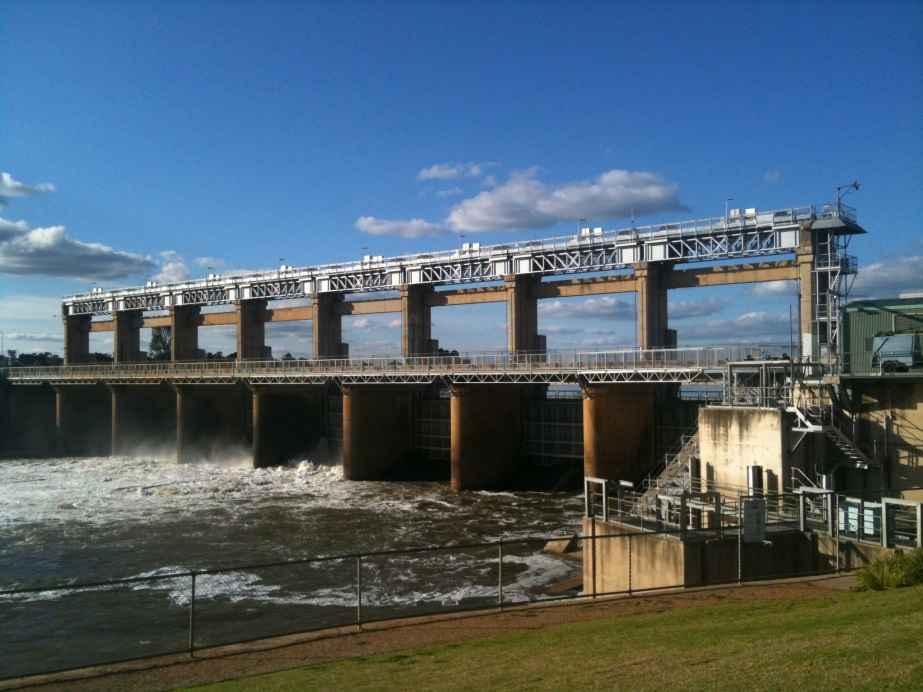
\includegraphics[width=8.4cm]{figs/intro/goolwa.jpg}
\caption{The Goolwa barrage}
\label{figs:intro:goolwa}
\end{figure}

Stoplogs are modular and manually operated. At inserting or removing process,
the operator of a gated structure controls the water
level in channel by adding or removing individual stoplogs with a lifiting beam.
However, problems may occur during the process: bad coupling between lifting
beam and stoplog, bad stoplog stacking due to sediments, and difficult removal
owing to silt particles accumulation and hydrostatic pressure. In the specific
case of Jirau power plant, in Rond{\^o}nia, Brazil, the Madeira River tears out
trees along the stretch, carrying more than 500 tons of sediments every day
\citep{amazon}.

\citet{jack} studies stoplogs and lifting beam's physical and
mechanical properties. The ideal stoplog, as mentioned in the book, has a
mechanical contact sensor, and an hydrostatic pressure regulator valve, which
solve most of the problems with stoplogs operation. However, in \cite{pinc},
England, a technical standard for stoplogs are proposed to manufacturing,
cost and maintenance reasons, without sensing technology. Regarding solving
stoplog installation problems, increasing efficiency and reducing downtime,
companies develop robotic systems, besides of the improvement in Health,
Safety, and Environment (HSE) conditions, as robots can replace humans in tasks
performed in unhealthy and hazardous areas.


%Guilherme: Senti falta de refs para a parte do subsea

The MIMROex inspection robot  was developed and
tested by the Fraunhofer Institute of Manufacturing Engineering and Automation
(IPA). The robot is capable o.f safely navigate in offshore environments, and
autonomously execute inspection tasks. Sensabot , a
teleoperated inspection robot developed by Carnegie Mellon University, was
designed for severe weather and atmosphere, being certified to operate in toxic, flammable and explosive environments. The SINTEF Topside Robotic System, developed in the robotic lab facility in
Trondheim, Norway, is an intelligent instrumentation system designed to enable onshore operators
to monitor and control the platform's processes .


%The robot includes the following sensors:
%\begin{enumerate}[i)]
%    \item Hydrocarbon sensor
%    \item Pan/tilt/zoom camera for remote operations
%    \item Temperature sensors
%    \item Vibration sensor for pumps, motors and bearings inspection
%    \item Microphone to detect audible machinery problems
%    \item Video camera to detect obstacles
%\end{enumerate}

 
%In this paper, we describe the DORIS project, which aims to develop a mobile
%robot to perform monitoring and inspection in an
%offshore platform. To this end, the system must be able to move throughout the
%monitored environment carrying different sensors, analyzing sensor data
%\emph{in loco} or storing it for a posterior analysis, and interpreting the
%results. The sensors can identify abnormalities such as intruders in restricted
%areas, abandoned objects, smoke, fire, and liquid and gas leakages.
%Furthermore, the robot is able to make machinery diagnosis, read instruments,
%and takes samples using an embedded manipulator (\cite{cba}).

In this paper, we present a general overview of the ROSA robot, and a detailed
description of the embedded electronics, power supply system and software
architecture. The robot is designed to perform monitoring and inspection tasks
in an offshore platform, being able to move throughout the monitored
environment carrying different sensors, analyzing sensor data \emph{in loco} or
storing it for a posterior analysis, and interpreting the results. The sensors
can identify abnormalities such as intruders in restricted areas, abandoned
objects, smoke, fire, and liquid and gas leakages.
The robot is able to make machinery diagnosis, read instruments, and takes
samples using an embedded manipulator (\cite{cba}).

This text is organized as follows: a general overview of the robot and its main
challenges are presented in Section \ref{sec:general_overview}, detailed
descriptions of the embedded electronics, the vehicle support system, power
supply system, and software architecture are taken in
Sections \ref{sec:electronics_overview}, \ref{sec:powersupply_overview}, and
\ref{sec:software} respectively.
In Section \ref{sec:results}, preliminary results are shown, and concluding
remarks are drawn in Section \ref{sec:conclusions}.